Ce projet interdisciplinaire, intitulé "AI Marketplace", consiste en la création d'une application de type Marketplace de l'AI basée sur un portefeuille de micro-services encapsulant des modèles machine-learning. Ces micro-services doivent être facilement interfaçables/assemblables pour créer des applications complètes. Pour donner un exemple concret, l’assemblage d’un module de détection d’objets dans une image, suivi par un module d'image captioning puis par un module text-to-speech permettrait de créer un service "lunettes AI pour malvoyant". 

Les projets doivent inclure différentes dimensions liées au Software Engineering (par exemple le design d'API REST OpenAPI) et au Data Science pour sélectionner et intégrer des modèles d'intelligence artificielle pertinents (NLP, image, parole, etc.). Des aspects DevOps et MLOps sont utilisées pour intégrer la mise à l’échelle des services AI (p.ex. déploiement Kubernetes) et pour faciliter une intégration continue de ces services (p.ex. MLFlow). Finalement, une interface utilisateur doit être proposée pour permettre à l’utilisateur final de sélectionner et d’assembler des pipelines de traitement des données par IA (p.ex. similaire à Knime). Chaque groupe doit donc imaginer un cas d'utilisation à mettre en place, représenté par une pipeline (chaînage) constituée de plusieurs micro-services qui peuvent être interfacés les uns aux autres pour effectuer une tâche globale. 

Notre projet consiste à créer de l'art sous forme d'image à partir d'une musique. Dans un cas concret, cette image pourrait par exemple être utilisée comme pochette de l'album. La pipeline complète composée des étapes intermédiaires pour réaliser ce cas d'utilisation est décrite par la figure \ref{fig:flowchart}. Chacune de ces étapes correspond à une tâche, qui sera exécutée par un micro-service spécifique, à savoir:

\begin{itemize}
    \item \textbf{Récupération de l'audio:} téléchargement d'un flux audio provenant de YouTube.
    \item \textbf{Reconnaissance de la parole:} analyse de la voix humaine d'un fichier audio et transcription sous forme textuelle.
    \item \textbf{Analyse de sujet/sentiment:} analyse d'un texte et extraction des sujets et/ou émotions qui y sont exprimés.
    \item \textbf{Détecteur de style de musique:} détection du style musicale d'un fichier audio caractérisant une musique.
    \item \textbf{Générateur d'art:} génération d'images à partir de données textuelles.
\end{itemize}

Notre pipeline pourra être exécutée, par l'utilisateur, au travers d'une application web lui permettant d'importer un fichier audio à traiter. Il recevra en réponse une ou plusieurs images caractérisant le style de sa musique et, si elle contient des paroles, les sujets ou sentiments qui y sont transmis.

Ce rapport est divisé en cinq chapitres. Dans un premier temps, les objectifs spécifiques à ce projet intégré sont présentés dans la section suivante. Ensuite, les aspects DevOps et MLOps intégrés au projet sont décrits, suivis des services implémentés ainsi que la pipeline complète les intégrant. Finalement, nous concluons le projet et proposons des perspectives d'améliorations.


\begin{figure}[H]
    \begin{center}
        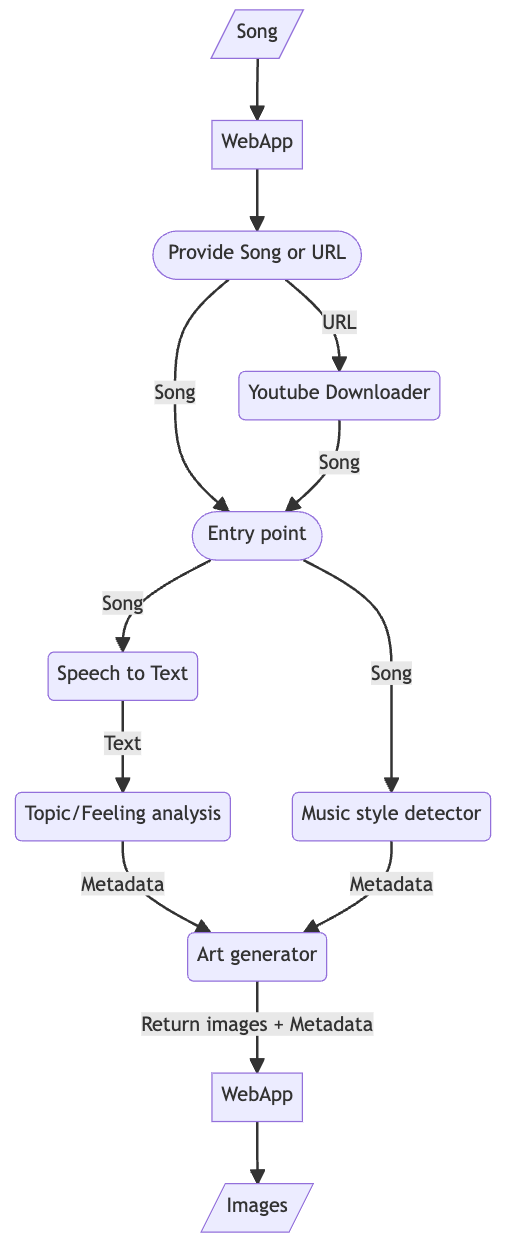
\includegraphics[height=22cm,]{rsc/flowchart.png}
        \caption{Flowchart du use case}
        \label{fig:flowchart}
    \end{center}
\end{figure}


\section{Objectifs}

En plus des \href{https://www.hes-so.ch/fileadmin/documents/HES-SO/Documents_HES-SO/pdf/ingenierie_architecture/master/Engineering_MSE/Descriptifs_Modules/MSE_-_Descriptif_de_module_-_Projets_Interdisciplinaires__PI__-_V2021-08-31.pdf}{objectifs fixés par le Master}, ce projet intégré en comporte d'autres plus spécifiques:

\begin{itemize}
    \item Avoir un ou plusieurs workflow(s) démontrable(s) en fin de projet; un workflow est composé au minimum de 2 micro-services;
    \item Utiliser des outils CI/CD pour le déploiement;
    \item Utiliser Kubernetes comme plate-forme de déploiement - ou autre plate-forme permettant la distribution et mise à l'échelle des calculs;
    \item Au moins un des modèles ML doit pouvoir être ré-entraînable automatiquement à travers les outils CI/CD (i.e. MLOps);
    \item Proposer une organisation du travail en groupe;
    \item Proposer individuellement un ensemble de compétences à développer lors du projet.
\end{itemize}
\vspace{5mm}

Les compétences individuelles à développer pour chacun des membres du projet sont les suivantes:

\begin{itemize}
    \item \textbf{Andrea}
    \begin{itemize}
        \item Approfondir les connaissances en machine-learning.
        \item Découvrir les pratiques MLOps pour la création, le ré-entraînement et le déploiement d’un modèle.
        \item Apprendre à utiliser le framework de frontend VueJS.
    \end{itemize}
    \item \textbf{Florian}
    \begin{itemize}
        \item Consolider les compétences en DevOps, notamment en utilisant la plateforme GitHub.
        \item Approfondir les connaissances en machine-learning notamment en ce qui concerne la reconnaissance de parole.
        \item Découvrir les pratiques MLOps.
    \end{itemize}
    \item \textbf{Benjamin}
    \begin{itemize}
        \item Découvrir et mettre en place les pratiques de MLOps.
        \item  Approfondir et consolider les compétences en terme de création, d’entraînement et d’évaluation d’un modèle de deep-learning ainsi que son encapsulation dans un micro-service.
    \end{itemize}
    \item \textbf{Thibaut}
    \begin{itemize}
        \item Découvrir et mettre en place un outil d’orchestration de workflow afin de connecter les différents micro-services.
        \item Découvrir la génération d’image et approfondir les connaissance en machine-learning ainsi que l’encapsulation d’un modèle dans un micro-service.
    \end{itemize}    
\end{itemize}



% Ce rapport décrit les différentes étapes de notre projet, de la conception à la réalisation, en passant par les choix technologiques et les difficultés rencontrées. Il est divisé en 3 parties principales:

% \begin{itemize}
%     \item \textbf{DevOps \& MLOps:} Cette partie décrit les choix technologiques et les outils utilisés pour la mise en place de l'infrastructure et des pipelines de CI/CD et MLOps. 
%     \item \textbf{Services:} Cette partie parle des différents micro-services de notre pipeline.
%     \item \textbf{Pipeline:} Cette partie relate de l'application web et de l'orchestrateur permettant d'exécuter notre pipeline.
    
% \end{itemize}

% Pour finir, une conclusion générale est proposée, ainsi que les perspectives d'amélioration et les difficultés rencontrées. Chaque membres du groupe a également rédigé une conclusion personnelle décrivant son travail et ses compétences acquises durant le projet.